% Options for packages loaded elsewhere
\PassOptionsToPackage{unicode}{hyperref}
\PassOptionsToPackage{hyphens}{url}
\PassOptionsToPackage{dvipsnames,svgnames,x11names}{xcolor}
%
\documentclass[
  10pt,
]{article}
\usepackage{amsmath,amssymb}
\usepackage{iftex}
\ifPDFTeX
  \usepackage[T1]{fontenc}
  \usepackage[utf8]{inputenc}
  \usepackage{textcomp} % provide euro and other symbols
\else % if luatex or xetex
  \usepackage{unicode-math} % this also loads fontspec
  \defaultfontfeatures{Scale=MatchLowercase}
  \defaultfontfeatures[\rmfamily]{Ligatures=TeX,Scale=1}
\fi
\usepackage{lmodern}
\ifPDFTeX\else
  % xetex/luatex font selection
\fi
% Use upquote if available, for straight quotes in verbatim environments
\IfFileExists{upquote.sty}{\usepackage{upquote}}{}
\IfFileExists{microtype.sty}{% use microtype if available
  \usepackage[]{microtype}
  \UseMicrotypeSet[protrusion]{basicmath} % disable protrusion for tt fonts
}{}
\makeatletter
\@ifundefined{KOMAClassName}{% if non-KOMA class
  \IfFileExists{parskip.sty}{%
    \usepackage{parskip}
  }{% else
    \setlength{\parindent}{0pt}
    \setlength{\parskip}{6pt plus 2pt minus 1pt}}
}{% if KOMA class
  \KOMAoptions{parskip=half}}
\makeatother
\usepackage{xcolor}
\usepackage[margin=0.85in]{geometry}
\usepackage{color}
\usepackage{fancyvrb}
\newcommand{\VerbBar}{|}
\newcommand{\VERB}{\Verb[commandchars=\\\{\}]}
\DefineVerbatimEnvironment{Highlighting}{Verbatim}{commandchars=\\\{\}}
% Add ',fontsize=\small' for more characters per line
\newenvironment{Shaded}{}{}
\newcommand{\AlertTok}[1]{\textcolor[rgb]{1.00,0.00,0.00}{\textbf{#1}}}
\newcommand{\AnnotationTok}[1]{\textcolor[rgb]{0.38,0.63,0.69}{\textbf{\textit{#1}}}}
\newcommand{\AttributeTok}[1]{\textcolor[rgb]{0.49,0.56,0.16}{#1}}
\newcommand{\BaseNTok}[1]{\textcolor[rgb]{0.25,0.63,0.44}{#1}}
\newcommand{\BuiltInTok}[1]{\textcolor[rgb]{0.00,0.50,0.00}{#1}}
\newcommand{\CharTok}[1]{\textcolor[rgb]{0.25,0.44,0.63}{#1}}
\newcommand{\CommentTok}[1]{\textcolor[rgb]{0.38,0.63,0.69}{\textit{#1}}}
\newcommand{\CommentVarTok}[1]{\textcolor[rgb]{0.38,0.63,0.69}{\textbf{\textit{#1}}}}
\newcommand{\ConstantTok}[1]{\textcolor[rgb]{0.53,0.00,0.00}{#1}}
\newcommand{\ControlFlowTok}[1]{\textcolor[rgb]{0.00,0.44,0.13}{\textbf{#1}}}
\newcommand{\DataTypeTok}[1]{\textcolor[rgb]{0.56,0.13,0.00}{#1}}
\newcommand{\DecValTok}[1]{\textcolor[rgb]{0.25,0.63,0.44}{#1}}
\newcommand{\DocumentationTok}[1]{\textcolor[rgb]{0.73,0.13,0.13}{\textit{#1}}}
\newcommand{\ErrorTok}[1]{\textcolor[rgb]{1.00,0.00,0.00}{\textbf{#1}}}
\newcommand{\ExtensionTok}[1]{#1}
\newcommand{\FloatTok}[1]{\textcolor[rgb]{0.25,0.63,0.44}{#1}}
\newcommand{\FunctionTok}[1]{\textcolor[rgb]{0.02,0.16,0.49}{#1}}
\newcommand{\ImportTok}[1]{\textcolor[rgb]{0.00,0.50,0.00}{\textbf{#1}}}
\newcommand{\InformationTok}[1]{\textcolor[rgb]{0.38,0.63,0.69}{\textbf{\textit{#1}}}}
\newcommand{\KeywordTok}[1]{\textcolor[rgb]{0.00,0.44,0.13}{\textbf{#1}}}
\newcommand{\NormalTok}[1]{#1}
\newcommand{\OperatorTok}[1]{\textcolor[rgb]{0.40,0.40,0.40}{#1}}
\newcommand{\OtherTok}[1]{\textcolor[rgb]{0.00,0.44,0.13}{#1}}
\newcommand{\PreprocessorTok}[1]{\textcolor[rgb]{0.74,0.48,0.00}{#1}}
\newcommand{\RegionMarkerTok}[1]{#1}
\newcommand{\SpecialCharTok}[1]{\textcolor[rgb]{0.25,0.44,0.63}{#1}}
\newcommand{\SpecialStringTok}[1]{\textcolor[rgb]{0.73,0.40,0.53}{#1}}
\newcommand{\StringTok}[1]{\textcolor[rgb]{0.25,0.44,0.63}{#1}}
\newcommand{\VariableTok}[1]{\textcolor[rgb]{0.10,0.09,0.49}{#1}}
\newcommand{\VerbatimStringTok}[1]{\textcolor[rgb]{0.25,0.44,0.63}{#1}}
\newcommand{\WarningTok}[1]{\textcolor[rgb]{0.38,0.63,0.69}{\textbf{\textit{#1}}}}
\usepackage{longtable,booktabs,array}
\usepackage{calc} % for calculating minipage widths
% Correct order of tables after \paragraph or \subparagraph
\usepackage{etoolbox}
\makeatletter
\patchcmd\longtable{\par}{\if@noskipsec\mbox{}\fi\par}{}{}
\makeatother
% Allow footnotes in longtable head/foot
\IfFileExists{footnotehyper.sty}{\usepackage{footnotehyper}}{\usepackage{footnote}}
\makesavenoteenv{longtable}
\usepackage{graphicx}
\makeatletter
\def\maxwidth{\ifdim\Gin@nat@width>\linewidth\linewidth\else\Gin@nat@width\fi}
\def\maxheight{\ifdim\Gin@nat@height>\textheight\textheight\else\Gin@nat@height\fi}
\makeatother
% Scale images if necessary, so that they will not overflow the page
% margins by default, and it is still possible to overwrite the defaults
% using explicit options in \includegraphics[width, height, ...]{}
\setkeys{Gin}{width=\maxwidth,height=\maxheight,keepaspectratio}
% Set default figure placement to htbp
\makeatletter
\def\fps@figure{htbp}
\makeatother
\setlength{\emergencystretch}{3em} % prevent overfull lines
\providecommand{\tightlist}{%
  \setlength{\itemsep}{0pt}\setlength{\parskip}{0pt}}
\setcounter{secnumdepth}{-\maxdimen} % remove section numbering
\ifLuaTeX
  \usepackage{selnolig}  % disable illegal ligatures
\fi
\usepackage{bookmark}
\IfFileExists{xurl.sty}{\usepackage{xurl}}{} % add URL line breaks if available
\urlstyle{same}
\hypersetup{
  pdftitle={Prior-Relative Sparse Context: Knowledge Grams for Selective Activation of Model-Relative Memory},
  pdfauthor={{[}Author name(s) and affiliation(s) to be completed{]}},
  colorlinks=true,
  linkcolor={Maroon},
  filecolor={Maroon},
  citecolor={Blue},
  urlcolor={Blue},
  pdfcreator={LaTeX via pandoc}}

\title{Prior-Relative Sparse Context: Knowledge Grams for Selective
Activation of Model-Relative Memory}
\author{{[}Author name(s) and affiliation(s) to be completed{]}}
\date{Version 0.1 --- 15 November 2026}

\begin{document}
\maketitle

\section{Abstract}\label{abstract}

Large language models (LLMs) repeatedly process long contexts that
contain a mixture of familiar structure, corpus-specific facts,
exceptions, and relationships. Existing approaches reduce this cost
through prompt compression, learned latent context, corpus-specific
memory, retrieval, or reuse and transport of key-value (KV) caches. We
propose \textbf{Prior-Relative Sparse Context (PRSC)}, an architecture
that represents an external knowledge archive relative to a fixed base
model. PRSC compiles source material into addressable \textbf{Knowledge
Grams (K-grams)}: typed records that reference reusable patterns, encode
instance-specific residuals, preserve provenance and relationships, and
optionally point to compatible precomputed neural representations. At
query time, a retrieval-and-activation controller selects a small,
task-relevant working set, expands dependencies as needed, and loads
compatible cached representations or reconstructs them from a canonical
pattern plus residual. The archive remains external; only the active
working set enters model computation.

The central hypothesis is not that arbitrary context can be losslessly
reduced to logarithmic size. Rather, for workloads with repeated
structure and localized queries, PRSC may make lookup sublinear in
archive size and active context proportional to the information actually
needed, while preserving task quality. We formalize this objective,
describe a compilation and inference pipeline, specify compatibility and
correctness constraints for KV activation, and propose an evaluation
against full-context, retrieval, compression, and precomputed-cache
baselines. No empirical results are claimed. The contribution is an
architecture and research agenda for testing whether model-relative
residuals can complement existing context-memory systems.

\textbf{Keywords:} long-context inference, context compression, external
memory, key-value cache, retrieval-augmented generation, model-relative
encoding, sparse activation, knowledge representation

\section{1. Introduction}\label{introduction}

An LLM's context is often treated as a linear sequence that must be
prefetched into the model before generation. This is a useful interface,
but it is not necessarily the right storage abstraction for a large,
persistent knowledge base. A code repository, a technical manual, or a
long-running project history contains repeated conventions and
structures alongside the few facts that are specific to that corpus. A
model may already possess useful general competence about the
conventions, but still needs access to exact names, values, exceptions,
dependencies, and provenance.

This motivates a question: \textbf{can a context archive be represented
primarily by references to structures that a model can already
interpret, plus the residual information that distinguishes each
instance?} If so, a query might activate only a small subset of the
archive rather than repeatedly encoding the entire archive.

We call this architecture \textbf{Prior-Relative Sparse Context (PRSC)}.
Its atomic representation is a \textbf{Knowledge Gram (K-gram)}: a
versioned, addressable unit that contains (i) a reference to a reusable
pattern or semantic structure, (ii) the residual payload required to
identify the particular instance, (iii) typed relationships to other
grams, (iv) provenance and exact-source fallback, and (v) optional
references to precomputed model-specific representations such as
KV-cache segments.

PRSC is deliberately a hybrid design. A pattern reference is not assumed
to be a magical pointer into an LLM's distributed weights. Neural
parameters generally do not expose a stable, explicit address for a
concept or template. PRSC therefore introduces a typed pattern catalogue
and a model-conditioned encoder/decoder that learns to map incoming
material to that catalogue. For patterns that are not safely represented
by the base model, the system stores a larger residual or the original
source. When a query requires exact detail, the system can expand a gram
or retrieve the canonical source instead of trusting an aggressively
compressed representation.

The proposal combines and extends several established lines of work.
Gisting compresses prompts into reusable learned activations {[}1{]}.
Memorizing Transformers retrieve prior internal representations through
approximate nearest-neighbor memory {[}2{]}. Cartridges learn
corpus-specific KV representations offline and reuse them at inference
time {[}3{]}. Latent Context Language Models (LCLMs) compress long
inputs into latent sequences and support adaptive expansion of relevant
segments {[}4{]}. TurboRAG precomputes chunk-level KV caches and
composes them for retrieval {[}5{]}, while CacheGen compresses and
streams KV caches {[}6{]}. These results establish important building
blocks; they do not, by themselves, establish the PRSC hypothesis that
residuals relative to a model-specific pattern catalogue are a useful
general-purpose representation.

\subsection{1.1 Contributions}\label{contributions}

This paper makes five proposal-level contributions:

\begin{enumerate}
\def\labelenumi{\arabic{enumi}.}
\tightlist
\item
  \textbf{A model-relative memory abstraction.} We define a K-gram as a
  structured reference-plus-residual record, with explicit provenance,
  uncertainty, compatibility, and source fallback.
\item
  \textbf{A compilation and activation architecture.} We describe how a
  frozen base model, a trainable encoder, a pattern catalogue, a graph
  index, and a cache manager can cooperate without modifying the base
  model's weights for every new archive.
\item
  \textbf{A task-preserving objective.} We formulate compression in
  terms of preserving query-conditioned task behavior rather than
  reconstructing every source token by default.
\item
  \textbf{A qualified complexity target.} We separate archive lookup,
  active-set size, prefill, and generation costs, and explain why
  logarithmic total context cost is not generally achievable.
\item
  \textbf{A falsifiable evaluation plan.} We specify baselines,
  ablations, benchmarks, metrics, and failure tests. We do not claim a
  working implementation or measured performance.
\end{enumerate}

\subsection{1.2 Scope and terminology}\label{scope-and-terminology}

PRSC concerns external, persistent context for a fixed or explicitly
versioned base model. It does not claim to shrink the model's parameter
count, make model knowledge perfectly addressable, or eliminate the need
to store unpredictable new facts. ``Prior-relative'' means that the
encoder is conditioned on a particular model and its known capabilities;
it does not mean that the model's weights are an exact symbolic
dictionary. ``Sparse context'' means that only a query-specific subset
is activated into the model's working memory. We write ``K-gram'' as
shorthand for ``Knowledge Gram''; it is not the conventional NLP term
\emph{k-gram}, which denotes a contiguous sequence of k tokens or
symbols. ``Logarithmic'' refers only to a possible index-lookup target
under stated data-structure assumptions, not to a universal bound on
storage, reasoning, or attention computation.

\section{2. Background and Related
Work}\label{background-and-related-work}

\subsection{2.1 Prompt compression and learned latent
context}\label{prompt-compression-and-learned-latent-context}

LLMLingua uses a coarse-to-fine strategy to remove less useful prompt
tokens while attempting to preserve task-relevant information {[}7{]}.
Gisting trains a model to compress prompts into a smaller set of
reusable activation-bearing gist tokens {[}1{]}. Both illustrate that a
long textual representation can sometimes be replaced by a smaller
model-consumable representation. However, prompt compression alone does
not necessarily create a persistent, addressable archive with explicit
residual fields, typed dependencies, source provenance, and independent
activation of subparts.

LCLMs revisit encoder-decoder context compression at scale and report
models trained at 1:4, 1:8, and 1:16 compression ratios. Their agent
design can skim compressed context and adaptively expand relevant
segments {[}4{]}. This is close to PRSC's coarse-to-fine activation
path. PRSC differs in making the representation a versioned collection
of individually addressable semantic records, with references to a
shared pattern catalogue and optional precomputed cache entries.

Cartridges provide an especially close precedent. They are smaller
corpus-specific KV representations trained offline through synthetic
conversations and context distillation; the reported results include
substantial memory and throughput improvements and inference-time
composition {[}3{]}. PRSC does not claim that corpus-specific KV memory
is new. Its question is whether an explicit model-relative residual
layer can improve composability, update granularity, provenance, and
selectivity beyond a corpus-level distilled representation.

\subsection{2.2 External memory and test-time
learning}\label{external-memory-and-test-time-learning}

Memorizing Transformers add approximate nearest-neighbor memory over
internal key-value representations and show that a model can use
information introduced at inference time, including newly defined
functions and theorems {[}2{]}. Titans introduce a learned long-term
neural memory that complements attention's shorter-term context {[}8{]}.
These approaches reinforce the idea that the active context window need
not be the only place where useful information lives. PRSC instead
emphasizes externally addressable, inspectable, versioned records and
residual encoding against a model-conditioned pattern catalogue.

\subsection{2.3 KV-cache reuse, composition, and
streaming}\label{kv-cache-reuse-composition-and-streaming}

TurboRAG precomputes chunk-level KV caches and stitches retrieved chunks
using independent-attention and reordered-RoPE techniques {[}5{]}.
CacheGen encodes KV caches into compact bitstreams and streams them
according to network conditions {[}6{]}. SCBench evaluates the KV-cache
lifecycle, including generation, compression, retrieval, and loading
{[}9{]}. A 2026 preprint studies editable and composable KV-cache notes
{[}10{]}. These works make on-demand activation technically plausible,
but cache reuse has strict compatibility constraints: model weights,
tokenizer, positional scheme, attention implementation, layer layout,
quantization, and the conditioning context can all matter. PRSC treats
cache compatibility as an explicit validation gate, not as an
assumption.

\subsection{2.4 Positioning}\label{positioning}

\begin{longtable}[]{@{}
  >{\raggedright\arraybackslash}p{(\columnwidth - 4\tabcolsep) * \real{0.3333}}
  >{\raggedright\arraybackslash}p{(\columnwidth - 4\tabcolsep) * \real{0.3333}}
  >{\raggedright\arraybackslash}p{(\columnwidth - 4\tabcolsep) * \real{0.3333}}@{}}
\toprule\noalign{}
\begin{minipage}[b]{\linewidth}\raggedright
Line of work
\end{minipage} & \begin{minipage}[b]{\linewidth}\raggedright
What it establishes
\end{minipage} & \begin{minipage}[b]{\linewidth}\raggedright
PRSC's proposed addition
\end{minipage} \\
\midrule\noalign{}
\endhead
\bottomrule\noalign{}
\endlastfoot
Prompt compression (e.g., LLMLingua) & Remove or rewrite prompt content
& Persistent, typed records with source fallback and relationships \\
Gist/latent context & Encode context into shorter learned
representations & Fine-grained references and residual payloads relative
to a model-specific catalogue \\
Cartridges & Reusable corpus-specific KV memory & Decomposed,
independently addressable knowledge units and explicit residuals \\
External neural memory & Retrieve information from persistent memory &
Human-inspectable provenance, versioning, and exact-source recovery \\
Precomputed KV retrieval/streaming & Reuse or transport neural cache
states & A controller that chooses among cache loading, regeneration,
and source expansion \\
\end{longtable}

This is a positioning against selected relevant work, not an exhaustive
novelty or priority survey. The proposed combination may overlap with
concurrent or unreviewed work not covered here.

\section{3. Problem Formulation}\label{problem-formulation}

Let:

\begin{itemize}
\tightlist
\item
  \(M\) be a frozen base model with a specified model and tokenizer
  revision;
\item
  \(X\) be an external archive, such as a repository or document
  collection;
\item
  \(Q\) be a query or task sampled from workload distribution
  \(\mathcal{D}_Q\);
\item
  \(Y\) be the desired task output;
\item
  \(Z=E_\phi(X;M)\) be the PRSC representation produced by encoder
  \(E_\phi\);
\item
  \(A(Z,Q;M)\) be the query-conditioned active representation produced
  by an activation controller.
\end{itemize}

A conventional full-context system computes an output using the entire
or a large portion of \(X\). PRSC instead seeks to produce a compact
persistent representation \(Z\) and activate only \(Z_Q=A(Z,Q;M)\).

The target is task preservation:

\[
\min_{E_\phi,A} \; \mathbb{E}_{Q\sim\mathcal{D}_Q}
\left[\mathcal{L}_{task}\left(P_M(\cdot\mid X,Q),P_M(\cdot\mid Z_Q,Q)\right)\right]
+ \lambda_s S(Z) + \lambda_a C(A(Z,Q;M)).
\]

Here \(S(Z)\) measures persistent storage and \(C\) measures query-time
activation cost. The loss may be task-specific: exact symbol resolution,
answer correctness, code-test pass rate, or divergence between the
full-context and compressed-context output distributions. The weights
\(\lambda_s\) and \(\lambda_a\) express storage and latency trade-offs.

A complementary distillation-style constraint is:

\[
D\left(P_M(Y\mid X,Q),P_M(Y\mid Z_Q,Q)\right)\leq\epsilon,
\]

where \(D\) measures a task-appropriate discrepancy. This is a design
objective, not a guarantee that a learned encoder can satisfy it for
arbitrary corpora and queries.

\subsection{3.1 Why model-relative residuals may
help}\label{why-model-relative-residuals-may-help}

If a base model already represents a reusable structure well, encoding
every instance as raw text can duplicate information. PRSC attempts to
factor an instance into a catalogue reference and an instance-specific
residual:

\[
X_i \rightsquigarrow (p_i, r_i, e_i),
\]

where \(p_i\) is a pattern reference, \(r_i\) is residual information,
and \(e_i\) contains links and evidence. This is a conceptual
factorization, not literal subtraction in weight space. The catalogue
may contain symbolic templates, learned latent prototypes, canonical
prompt fragments, or model-specific activation recipes.

The central uncertainty is whether the pattern reference can be made
compact and reusable without hiding important information in opaque
latent state. PRSC therefore keeps source spans and confidence values,
and should escalate to a larger residual or original-source retrieval
whenever confidence is low or exactness is required.

\subsection{3.2 Lower bounds and
non-goals}\label{lower-bounds-and-non-goals}

If an archive contains \(B\) independent, unpredictable bits that are
not represented in \(M\), a system cannot losslessly encode all of them
in substantially fewer than \(B\) bits without additional assumptions.
Model-relative compression is useful only to the extent that the archive
contains redundancy, predictable structure, or information irrelevant to
the workload.

PRSC does not promise:

\begin{itemize}
\tightlist
\item
  lossless reconstruction of every source token from a tiny residual;
\item
  logarithmic storage in total archive size;
\item
  constant-size active context for tasks requiring broad global
  comparison;
\item
  universal KV-cache portability across models or positions;
\item
  safe compression based only on language-model surprisal or semantic
  similarity.
\end{itemize}

\section{4. Architecture}\label{architecture}

Figure 1 shows the proposed pipeline. The persistent archive is external
to the base model. The compiler produces K-grams and a graph/index. A
query-time controller retrieves a candidate set, expands required
dependencies, validates cache compatibility, and constructs an active
working set. It may load precomputed KV data, reconstruct a
representation from a canonical pattern and residual, or fall back to
exact source text.

\begin{figure}
\centering
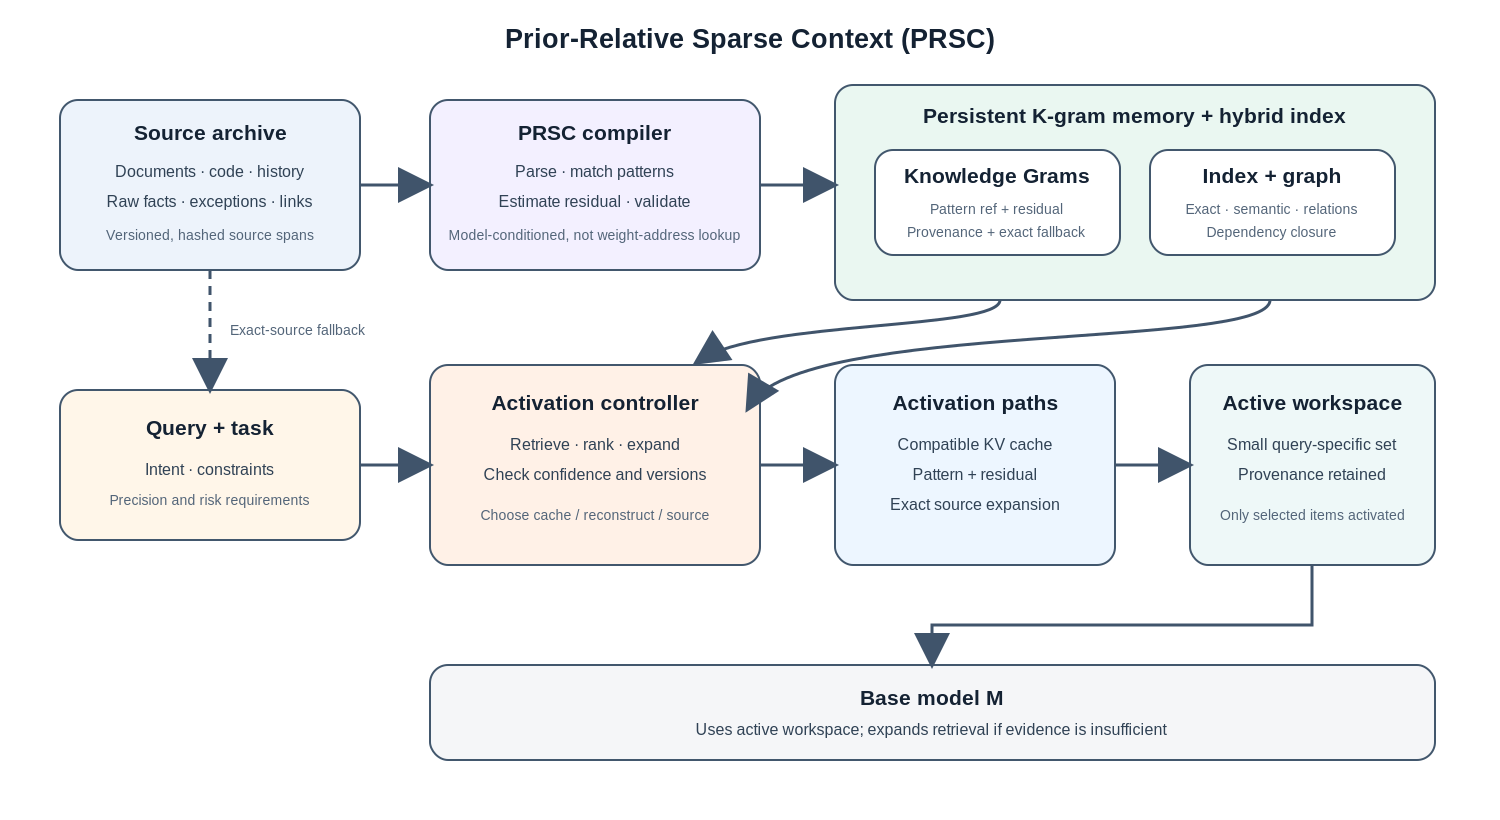
\includegraphics[width=0.95\textwidth,height=\textheight]{figures/prsc-architecture.png}
\caption{PRSC architecture: source archive to compiler, K-gram memory
and index, query controller, cache activation and source fallback, then
active model workspace.}
\end{figure}

\subsection{4.1 Components}\label{components}

\textbf{Base model \(M\).} A pretrained model with fixed, recorded
weights and tokenizer revision. PRSC does not assume that concepts have
direct addresses in its weights.

\textbf{Pattern catalogue \(P_M\).} A versioned collection of typed
reusable structures. Entries may be symbolic patterns (AST templates,
API schemas, semantic frames), trained latent prototypes, or canonical
conditioning snippets. Each entry declares the tasks and modalities for
which it is valid, and the model revisions for which its activations
were tested.

\textbf{Knowledge encoder \(E_\phi\).} Parses source material,
identifies candidate structures, estimates novelty and task-criticality,
aligns segments to catalogue entries, and emits residual payloads. It
should preserve exact identifiers, numbers, negations, exceptions,
temporal facts, and low-confidence spans rather than compress them away.

\textbf{K-gram store.} Stores records and payloads in a durable external
archive. It supports independent updates and retains provenance, source
hashes, timestamps, access labels, and exact-source fallback.

\textbf{Hierarchical index.} Combines exact-key and symbol indexes,
lexical or dense retrieval, and a relationship graph. Exact indexes
serve identifiers and known entities; semantic retrieval identifies
candidate concepts; graph traversal follows dependencies and references.

\textbf{Activation controller.} Ranks candidate grams by expected task
utility per unit cost, computes a dependency closure where necessary,
checks uncertainty and compatibility, and decides whether to load a
cache, reconstruct a representation, or expand original source.

\textbf{Cache manager.} Stores optional model-specific KV segments or
other neural representations. Cache manifests contain a model
fingerprint, tokenizer fingerprint, cache format, positional metadata,
layer layout, quantization configuration, and provenance. A mismatch
must invalidate reuse or trigger explicit adaptation/recomputation.

\textbf{Active workspace.} The currently materialized K-grams, source
expansions, and compatible KV entries. It is the only part of the
archive intended to occupy the model's active context or device memory
for the current query.

\subsection{4.2 Knowledge Gram data
model}\label{knowledge-gram-data-model}

A K-gram is an addressable record, not necessarily a single token
sequence. A minimal record has:

\begin{longtable}[]{@{}
  >{\raggedright\arraybackslash}p{(\columnwidth - 2\tabcolsep) * \real{0.5000}}
  >{\raggedright\arraybackslash}p{(\columnwidth - 2\tabcolsep) * \real{0.5000}}@{}}
\toprule\noalign{}
\begin{minipage}[b]{\linewidth}\raggedright
Field
\end{minipage} & \begin{minipage}[b]{\linewidth}\raggedright
Purpose
\end{minipage} \\
\midrule\noalign{}
\endhead
\bottomrule\noalign{}
\endlastfoot
\texttt{gram\_id} & Stable identifier within an archive namespace \\
\texttt{model\_compatibility} & Base-model, tokenizer, adapter, and
encoder fingerprints \\
\texttt{pattern\_ref} & Typed reference to a catalogue structure \\
\texttt{residual} & Symbolic, textual, latent, or patch-like
instance-specific payload \\
\texttt{relations} & Typed links to other K-grams, including required
dependencies \\
\texttt{provenance} & Source URI, span, content hash, and update
metadata \\
\texttt{activation} & Preferred activation path and optional cache
manifest \\
\texttt{confidence} & Calibrated estimate of safe reuse for declared
tasks \\
\texttt{exact\_fallback} & Pointer to the original source or an
independently verifiable payload \\
\end{longtable}

The example in \texttt{examples/knowledge-gram.example.json} and schema
in \texttt{schemas/knowledge-gram.schema.json} define a candidate
serialization. The schema is illustrative and can evolve before
implementation.

\subsection{4.3 Compile-time workflow}\label{compile-time-workflow}

\begin{enumerate}
\def\labelenumi{\arabic{enumi}.}
\tightlist
\item
  \textbf{Ingest and fingerprint.} Split the archive into
  source-addressable units; preserve stable IDs and cryptographic
  hashes.
\item
  \textbf{Parse and annotate.} Use modality-specific parsers where
  possible (e.g., ASTs and symbol tables for code; entities, relations,
  and document structure for prose).
\item
  \textbf{Match patterns.} Retrieve candidate catalogue entries using
  exact structural matching and model-conditioned semantic matching.
\item
  \textbf{Estimate residuals.} Encode the parts not safely covered by
  the candidate pattern. Preserve task-critical details, exceptions, and
  provenance.
\item
  \textbf{Build relations.} Add explicit dependency, reference,
  containment, temporal, and contradiction edges.
\item
  \textbf{Validate.} Reconstruct sampled source units, test behavioral
  invariants, and reject unsafe compression. Keep exact-source fallback.
\item
  \textbf{Optionally precompute activations.} Generate KV
  representations only for reusable units with a well-defined canonical
  conditioning context and supported cache semantics.
\item
  \textbf{Index and publish.} Store the K-grams, indexes, cache
  manifests, and archive version atomically.
\end{enumerate}

\subsection{4.4 Query-time activation}\label{query-time-activation}

For a query \(Q\), the controller:

\begin{enumerate}
\def\labelenumi{\arabic{enumi}.}
\tightlist
\item
  classifies the task and extracts exact identifiers, constraints, and
  requested precision;
\item
  retrieves candidate grams using exact, lexical, semantic, and graph
  indexes;
\item
  estimates the utility and confidence of each candidate;
\item
  expands required dependencies and checks for contradictions or stale
  versions;
\item
  selects a representation path for each gram: cached KV, reconstructed
  latent/symbolic representation, or exact-source expansion;
\item
  validates model/cache compatibility before loading neural states;
\item
  assembles a small active workspace and exposes provenance to the
  answer generator;
\item
  monitors for uncertainty or evidence of a missing dependency, then
  retrieves more context if needed.
\end{enumerate}

This makes activation adaptive rather than fixed top-k retrieval. A
query about one function may activate only a few grams; a query about a
global architectural property may require a much larger dependency
closure or even the whole archive.

\section{5. Algorithms and Training
Objectives}\label{algorithms-and-training-objectives}

\subsection{5.1 Compilation algorithm}\label{compilation-algorithm}

\begin{Shaded}
\begin{Highlighting}[]
\NormalTok{COMPILE(archive X, base model M, pattern catalogue P\_M):}
\NormalTok{    units \textless{}{-} source\_aware\_partition\_and\_parse(X)}
\NormalTok{    grams \textless{}{-} []}
\NormalTok{    for unit in units:}
\NormalTok{        candidates \textless{}{-} MATCH\_PATTERNS(unit, P\_M)}
\NormalTok{        pattern \textless{}{-} select candidate using structural fit and calibrated confidence}
\NormalTok{        if pattern is absent or confidence is insufficient:}
\NormalTok{            residual \textless{}{-} preserve unit at a conservative fidelity level}
\NormalTok{            pattern\_ref \textless{}{-} null}
\NormalTok{        else:}
\NormalTok{            residual \textless{}{-} ENCODE\_RESIDUAL(unit, pattern)}
\NormalTok{            pattern\_ref \textless{}{-} pattern.id}
\NormalTok{        relations \textless{}{-} EXTRACT\_RELATIONS(unit, units)}
\NormalTok{        evidence \textless{}{-} RECORD\_PROVENANCE(unit, X)}
\NormalTok{        if not VALIDATE\_RECONSTRUCTION(unit, pattern\_ref, residual):}
\NormalTok{            residual \textless{}{-} exact\_or\_high\_fidelity\_payload(unit)}
\NormalTok{        grams.append(K\_GRAM(pattern\_ref, residual, relations, evidence))}
\NormalTok{    index \textless{}{-} BUILD\_HYBRID\_INDEX(grams)}
\NormalTok{    caches \textless{}{-} OPTIONAL\_PRECOMPUTE\_COMPATIBLE\_ACTIVATIONS(grams, M)}
\NormalTok{    return COMMIT\_VERSIONED\_ARCHIVE(grams, index, caches)}
\end{Highlighting}
\end{Shaded}

The routine is deliberately conservative: a pattern match is not enough
to discard the source. The encoder must demonstrate reconstruction or
task preservation on the relevant validation cases.

\subsection{5.2 Activation algorithm}\label{activation-algorithm}

\begin{Shaded}
\begin{Highlighting}[]
\NormalTok{ACTIVATE(query Q, archive Z, base model M, budget B):}
\NormalTok{    intent \textless{}{-} ANALYZE\_QUERY(Q)}
\NormalTok{    candidates \textless{}{-} HYBRID\_RETRIEVE(Z.index, intent)}
\NormalTok{    candidates \textless{}{-} ADD\_REQUIRED\_DEPENDENCIES(candidates, Z.graph)}
\NormalTok{    ranked \textless{}{-} RANK\_BY\_EXPECTED\_UTILITY\_PER\_COST(candidates, intent)}
\NormalTok{    active \textless{}{-} []}
\NormalTok{    for gram in ranked:}
\NormalTok{        if budget\_exceeded(active, gram, B):}
\NormalTok{            break}
\NormalTok{        if cache\_manifest\_compatible(gram, M):}
\NormalTok{            item \textless{}{-} LOAD\_PRECOMPUTED\_ACTIVATION(gram)}
\NormalTok{        elif reconstruction\_is\_confident(gram, intent):}
\NormalTok{            item \textless{}{-} RESOLVE\_PATTERN\_AND\_RESIDUAL(gram)}
\NormalTok{        else:}
\NormalTok{            item \textless{}{-} EXPAND\_EXACT\_SOURCE(gram)}
\NormalTok{        active.append(VERIFY\_AND\_ATTACH\_PROVENANCE(item, gram))}
\NormalTok{    if insufficient\_evidence(active, intent):}
\NormalTok{        active \textless{}{-} EXPAND\_RETRIEVAL\_OR\_SOURCE(active, intent)}
\NormalTok{    return BUILD\_ACTIVE\_WORKSPACE(active)}
\end{Highlighting}
\end{Shaded}

The activation budget is a soft constraint. If the controller cannot
answer reliably under the budget, it should expand the working set or
report that the evidence is insufficient rather than silently omit
necessary information.

\subsection{5.3 Training objective}\label{training-objective}

A practical encoder and pattern catalogue could be trained with a
multi-objective loss:

\[
\mathcal{L} = \mathcal{L}_{task}
+ \lambda_r \mathcal{L}_{rate}
+ \lambda_x \mathcal{L}_{reconstruct}
+ \lambda_p \mathcal{L}_{provenance}
+ \lambda_c \mathcal{L}_{calibration}
+ \lambda_a \mathcal{L}_{activation}.
\]

\begin{itemize}
\tightlist
\item
  \(\mathcal{L}_{task}\): preserve task outputs or behavior under a
  workload distribution.
\item
  \(\mathcal{L}_{rate}\): penalize archive size and active-set cost.
\item
  \(\mathcal{L}_{reconstruct}\): preserve exact or behaviorally
  important details where required.
\item
  \(\mathcal{L}_{provenance}\): ensure each claim or residual can be
  traced to source evidence.
\item
  \(\mathcal{L}_{calibration}\): align confidence with empirical failure
  probability.
\item
  \(\mathcal{L}_{activation}\): optimize retrieval and expansion
  decisions under realistic latency and bandwidth budgets.
\end{itemize}

The training data must include adversarially similar examples, rare
identifiers, negative conditions, version changes, and exceptions.
Optimizing token-level surprisal alone is inadequate because a
low-surprisal token can be essential (for example, a negation, a version
number, or a single changed argument name).

\section{6. Complexity Analysis and the Logarithmic
Hypothesis}\label{complexity-analysis-and-the-logarithmic-hypothesis}

Let \(N\) be the number of indexed grams, \(S\) the total bytes in the
persistent archive, and \(k\) the number of grams activated for a query.
A useful query cost decomposition is:

\[
T_{query} = T_{lookup}(N) + T_{expand}(k) + T_{load}(k) + T_{prefill}(k) + T_{decode}(Q,Y).
\]

Under a balanced B-tree or similar exact index, a lookup can require
\(O(\log N)\) index steps. Graph expansion is output-sensitive and may
be closer to \(O(k + e_k)\), where \(e_k\) is the number of traversed
relations. Approximate nearest-neighbor indexes can be sublinear in
practice, but their guarantees depend on the index, data distribution,
and recall target; PRSC does not assume a universal logarithmic bound
for dense retrieval.

The desired regime is therefore:

\begin{itemize}
\tightlist
\item
  \textbf{Persistent storage:} proportional to the information that must
  actually be retained; not generally logarithmic in archive size.
\item
  \textbf{Index lookup:} logarithmic for suitable exact indexes, or
  empirical sublinear behavior for approximate retrieval.
\item
  \textbf{Active memory:} proportional to the query-specific working set
  \(k\), not the full archive \(N\).
\item
  \textbf{Prefill and decode:} depend on the activated representations
  and model architecture; exact attention and broad global tasks can
  still be expensive.
\end{itemize}

A small \(k\) is possible when queries are local and the archive has
reusable structure. It is not possible to promise small \(k\) for tasks
that genuinely require inspecting many independent records. The proper
claim is \textbf{sparse activation with potentially logarithmic archive
lookup}, not logarithmic total context computation.

\section{7. Correctness, Cache Compatibility, and
Safety}\label{correctness-cache-compatibility-and-safety}

\subsection{7.1 Cache compatibility is a hard
constraint}\label{cache-compatibility-is-a-hard-constraint}

A precomputed KV object must be treated as model-specific executable
state. At minimum, the manifest should bind it to:

\begin{itemize}
\tightlist
\item
  exact model weights and revision;
\item
  tokenizer and vocabulary revision;
\item
  adapter/LoRA stack and relevant routing configuration;
\item
  positional encoding and RoPE parameters;
\item
  attention implementation and layer/head layout;
\item
  cache dtype, quantization, page/block format, and serialization
  version;
\item
  canonical conditioning context and position semantics.
\end{itemize}

Even when tensor shapes match, the cache may be semantically
incompatible. Independently encoded chunks cannot simply be concatenated
unless the attention mask, position mapping, and inter-chunk
dependencies make that operation valid. Methods such as independent
attention, RoPE repositioning, or boundary recomputation are model- and
method-specific techniques, not universally safe transformations {[}5,
10{]}.

PRSC should initially use the conservative path: cache only
independently validated units, store a manifest, reject mismatches, and
fall back to text or latent recomputation. Cache composition can be
introduced incrementally with equivalence tests against full prefill.

\subsection{7.2 Exactness tiers}\label{exactness-tiers}

We propose three activation tiers:

\begin{itemize}
\tightlist
\item
  \textbf{Tier 0 --- exact source:} retrieve original bytes/tokens or a
  lossless symbolic representation; use for code execution, legal
  clauses, numeric facts, and audit-sensitive claims.
\item
  \textbf{Tier 1 --- validated structured reconstruction:} resolve a
  known pattern plus residual and validate the relevant fields or
  behavior.
\item
  \textbf{Tier 2 --- approximate latent activation:} use compressed
  activations when the task tolerates approximation and confidence is
  calibrated.
\end{itemize}

A controller must choose a tier based on task risk and requested
precision, not solely on a compression budget.

\subsection{7.3 Provenance and trust
boundaries}\label{provenance-and-trust-boundaries}

K-grams are data, not instructions. Retrieved source text may contain
prompt injection or malicious instructions. The generator must preserve
a strict separation between system instructions and untrusted archive
content. Provenance, content hashes, access controls, and version
histories are required to detect tampering and stale data. A gram with a
missing source, invalid hash, ambiguous ownership, or conflicting
versions should not be silently promoted to trusted memory.

\subsection{7.4 Privacy and deletion}\label{privacy-and-deletion}

The archive may contain sensitive material. It should support per-source
deletion, cryptographic erasure where appropriate, access-control
labels, retention policies, and cache invalidation. Deleting a source
requires deleting or rebuilding all derived grams, indexes, and KV
objects that depend on it; otherwise derived memory may preserve the
supposedly deleted information.

\section{8. Evaluation Plan}\label{evaluation-plan}

The first prototype should target software repositories, where
structures are explicit and correctness can be tested. A second phase
should test natural-language corpora and project histories.

\subsection{8.1 Research questions and
hypotheses}\label{research-questions-and-hypotheses}

\begin{itemize}
\tightlist
\item
  \textbf{RQ1 --- Compression:} Does model-relative
  pattern-plus-residual encoding reduce persistent and active memory at
  matched task quality compared with generic prompt compression and
  retrieval?
\item
  \textbf{RQ2 --- Reuse:} Does a shared pattern catalogue improve
  compression across multiple repositories or documents compared with
  independently learned corpus memories?
\item
  \textbf{RQ3 --- Activation:} Does graph-aware, confidence-triggered
  activation outperform fixed top-k retrieval on dependency-heavy
  questions?
\item
  \textbf{RQ4 --- KV reuse:} When does precomputed activation reduce
  time-to-first-token after accounting for cache storage, network
  transfer, and compatibility checks?
\item
  \textbf{RQ5 --- Robustness:} Which categories of facts, exceptions,
  edits, or adversarial examples are lost by compression, and can
  exact-source fallback recover them?
\end{itemize}

Pre-registered hypotheses:

\begin{itemize}
\tightlist
\item
  \textbf{H1:} At matched task quality, PRSC reduces active context or
  KV bytes for workloads with repeated patterns and local queries.
\item
  \textbf{H2:} A shared pattern catalogue improves storage amortization
  when the same structures recur across archives.
\item
  \textbf{H3:} Dependency-aware activation improves answer accuracy on
  cross-file and cross-document tasks relative to flat top-k retrieval
  at the same budget.
\item
  \textbf{H4:} Precomputed KV activation reduces TTFT only when reuse
  frequency and cache-transfer conditions amortize cache generation and
  storage costs.
\end{itemize}

These are hypotheses, not reported findings.

\subsection{8.2 Baselines}\label{baselines}

\begin{enumerate}
\def\labelenumi{\arabic{enumi}.}
\tightlist
\item
  \textbf{Full context:} all relevant source material provided to the
  base model, with the strongest feasible context window.
\item
  \textbf{Text RAG:} chunked retrieval followed by ordinary text
  prefill.
\item
  \textbf{Prompt compression:} LLMLingua or a comparable compressor
  {[}7{]}.
\item
  \textbf{Gist/latent context:} Gist Tokens or LCLM-style compression
  where available {[}1, 4{]}.
\item
  \textbf{Corpus-specific memory:} Cartridges-style corpus memory
  {[}3{]}.
\item
  \textbf{Precomputed KV retrieval:} TurboRAG-style cache retrieval
  {[}5{]}, with CacheGen-style transfer compression when applicable
  {[}6{]}.
\item
  \textbf{PRSC ablations:} remove the pattern catalogue, residual
  coding, graph edges, confidence gating, exact-source fallback, or KV
  activation one at a time.
\end{enumerate}

All baselines should use the same base model where feasible. If a
baseline requires a different model or retraining recipe, disclose that
mismatch and report both quality and systems costs.

\subsection{8.3 Workloads and datasets}\label{workloads-and-datasets}

Use a mix of controlled and realistic tasks:

\begin{itemize}
\tightlist
\item
  repository-level symbol and dependency questions;
\item
  exact retrieval of rare identifiers, constants, and version-specific
  behavior;
\item
  cross-file debugging and code change impact analysis;
\item
  repository question answering and patch generation with tests;
\item
  long-document fact retrieval, multi-document synthesis, and temporal
  contradiction resolution;
\item
  shared-context and KV-lifecycle evaluations such as SCBench {[}9{]};
\item
  long-context stress tests such as RULER or LongBench, with the exact
  model and configuration documented.
\end{itemize}

Repository corpora should include both repeated patterns and unique
facts. Synthetic cases should explicitly test negation, one-token
changes, stale versions, ambiguous references, and facts that are
statistically unsurprising but task-critical.

\subsection{8.4 Metrics}\label{metrics}

\begin{longtable}[]{@{}
  >{\raggedright\arraybackslash}p{(\columnwidth - 2\tabcolsep) * \real{0.5000}}
  >{\raggedright\arraybackslash}p{(\columnwidth - 2\tabcolsep) * \real{0.5000}}@{}}
\toprule\noalign{}
\begin{minipage}[b]{\linewidth}\raggedright
Category
\end{minipage} & \begin{minipage}[b]{\linewidth}\raggedright
Metric
\end{minipage} \\
\midrule\noalign{}
\endhead
\bottomrule\noalign{}
\endlastfoot
Task quality & Exact match, answer F1, code test pass rate, patch
acceptance, human preference \\
Compression & Source-to-archive bytes, gram payload bytes, active
tokens, active KV bytes \\
Retrieval & Recall@k, dependency recall, provenance coverage,
stale-reference rate \\
Systems & Index latency, compile cost, TTFT, decode throughput,
end-to-end latency, GPU/CPU memory, network bytes \\
Amortization & Queries-to-break-even, total cost over realistic
query-frequency distributions \\
Reliability & Calibration error, fallback frequency, false-compression
rate, silent omission rate \\
\end{longtable}

Report quality-versus-cost Pareto curves, not a single compression
ratio. Include the cost of compilation, cache storage, cache transfer,
graph maintenance, and fallback. A system that uses less active context
but requires expensive preprocessing may only win for repeatedly queried
archives.

\subsection{8.5 Essential ablations and failure
tests}\label{essential-ablations-and-failure-tests}

\begin{itemize}
\tightlist
\item
  Disable model-relative pattern references and retain residuals only.
\item
  Replace model-relative patterns with generic symbolic templates.
\item
  Remove relation edges and compare dependency recall.
\item
  Remove exact-source fallback and measure silent failure.
\item
  Vary the base model revision and verify invalidation behavior.
\item
  Test code with near-identical implementations that differ in one
  semantically critical token.
\item
  Test changing facts, source deletions, and conflicting versions.
\item
  Measure retrieval as archive size grows while holding query-local
  working-set size roughly fixed.
\item
  Compare cache reuse against recomputation under different network
  bandwidths and cache hit rates.
\end{itemize}

\section{9. Limitations and Open
Problems}\label{limitations-and-open-problems}

\textbf{Addressability of pretrained knowledge.} The model's internal
knowledge is distributed. A catalogue and encoder must learn a stable
interface to that knowledge; it cannot be assumed to exist natively.

\textbf{Domain and model dependence.} A pattern that is useful for one
model, tokenizer, or domain may not transfer. The pattern catalogue and
cached activations require versioning and regression tests.

\textbf{Residual estimation is difficult.} The difference between
``already known'' and ``new'' is query-dependent. A model can appear
familiar with a concept while lacking the exact detail needed for a
particular answer.

\textbf{Global tasks expand the working set.} Summaries, audits,
comparisons, and anomaly detection may require broad traversal. The
architecture reduces unnecessary work; it does not remove necessary
work.

\textbf{Cache composition is nontrivial.} KV states encode contextual
dependencies. A reusable cache must be independently meaningful or
transformed under a validated attention and positional scheme.

\textbf{Compilation can be expensive.} The benefit depends on archive
reuse frequency. A one-off query may be cheaper with ordinary text RAG.

\textbf{Evaluation is workload-sensitive.} Compression quality measured
on one query distribution may fail on another. A credible system must
disclose its supported tasks, test distribution shifts, and preserve
source fallback.

\section{10. Roadmap}\label{roadmap}

A staged research programme minimizes premature engineering:

\begin{enumerate}
\def\labelenumi{\arabic{enumi}.}
\tightlist
\item
  \textbf{Symbolic K-gram prototype:} parse code into functions,
  classes, symbols, and dependencies; use explicit templates plus
  structured residuals; retrieve exact source for generation.
\item
  \textbf{Model-relative encoder:} train an encoder to choose catalogue
  patterns and residual representations using task-preservation and
  exact-detail losses.
\item
  \textbf{Confidence-aware activation:} implement hybrid retrieval,
  dependency closure, confidence thresholds, and source fallback.
\item
  \textbf{Latent and KV activation:} add precomputed representations
  only after the symbolic system has passed correctness tests; validate
  against fresh prefill for every cache path.
\item
  \textbf{Cross-archive reuse:} measure whether common patterns amortize
  across multiple repositories or domains.
\item
  \textbf{Open evaluation:} publish configs, model fingerprints, corpus
  hashes where licensing allows, failure cases, and full cost
  accounting.
\end{enumerate}

\section{11. Conclusion}\label{conclusion}

PRSC proposes treating an LLM's external context as a persistent,
model-relative memory archive rather than a sequence that must always be
re-read. Knowledge Grams encode reusable pattern references,
instance-specific residuals, relationships, provenance, and optional
precomputed neural representations. A query-time controller activates a
small working set and expands to exact source when the task or
confidence requires it.

The proposal is intentionally more conservative than a claim of
``logarithmic context.'' Index lookup may be logarithmic under suitable
data structures, but total storage remains tied to the information that
must be retained, and broad tasks may require broad activation. The key
empirical question is whether a model-conditioned catalogue can reliably
separate reusable prior structure from the residual facts that
distinguish a particular archive. Existing work on Cartridges, latent
context, gist tokens, external memory, precomputed KV caches, and cache
streaming makes the components plausible. Whether their integration
yields a distinct and useful trade-off remains to be demonstrated.

\section{References}\label{references}

{[}1{]} Jesse Mu, Xiang Lisa Li, and Noah Goodman. ``Learning to
Compress Prompts with Gist Tokens.'' \emph{Advances in Neural
Information Processing Systems 36}, 2023.
https://arxiv.org/abs/2304.08467. DOI: 10.52202/075280-0848.

{[}2{]} Yuhuai Wu, Markus Rabe, DeLesley Hutchins, and Christian
Szegedy. ``Memorizing Transformers.'' \emph{International Conference on
Learning Representations}, 2022. https://arxiv.org/abs/2203.08913.

{[}3{]} Sabri Eyuboglu, Ryan Ehrlich, Simran Arora, Neel Guha, Dylan
Zinsley, Emily Liu, Atri Rudra, James Y. Zou, Azalia Mirhoseini, and
Christopher Ré. ``Cartridges: Lightweight and General-Purpose Long
Context Representations via Self-Study.'' \emph{International Conference
on Learning Representations}, 2026.
https://proceedings.iclr.cc/paper\_files/paper/2026/hash/4681359a7b1e94571598ad1adda35e6e-Abstract-Conference.html.

{[}4{]} Ang Li, Sean McLeish, Haozhe Chen, Nimit Kalra, Zaiqian Chen,
Artem Gazizov, Venkata Anoop Suhas Kumar Morisetty, Bhavya Kailkhura,
Harshitha Menon, Zhuang Liu, Brian R. Bartoldson, Tom Goldstein, Sanae
Lotfi, Micah Goldblum, and Pavel Izmailov. ``End-to-End Context
Compression at Scale.'' arXiv preprint arXiv:2606.09659, 2026.
https://arxiv.org/abs/2606.09659.

{[}5{]} Songshuo Lu, Hua Wang, Yutian Rong, Zhi Chen, and Yaohua Tang.
``TurboRAG: Accelerating Retrieval-Augmented Generation with Precomputed
KV Caches for Chunked Text.'' \emph{Proceedings of EMNLP 2025},
pp.~6588--6601. https://aclanthology.org/2025.emnlp-main.334/. DOI:
10.18653/v1/2025.emnlp-main.334.

{[}6{]} Yuhan Liu, Hanchen Li, Yihua Cheng, Siddhant Ray, Yuyang Huang,
Qizheng Zhang, Kuntai Du, Jiayi Yao, Shan Lu, Ganesh Ananthanarayanan,
Michael Maire, Henry Hoffmann, Ari Holtzman, and Junchen Jiang.
``CacheGen: KV Cache Compression and Streaming for Fast Large Language
Model Serving.'' \emph{Proceedings of ACM SIGCOMM 2024}, pp.~38--56.
https://doi.org/10.1145/3651890.3672274.

{[}7{]} Huiqiang Jiang, Qianhui Wu, Chin-Yew Lin, Yuqing Yang, and Lili
Qiu. ``LLMLingua: Compressing Prompts for Accelerated Inference of Large
Language Models.'' \emph{Proceedings of EMNLP 2023}, pp.~13358--13376.
https://aclanthology.org/2023.emnlp-main.825/. DOI:
10.18653/v1/2023.emnlp-main.825.

{[}8{]} Ali Behrouz, Peilin Zhong, and Vahab Mirrokni. ``Titans:
Learning to Memorize at Test Time.'' \emph{Advances in Neural
Information Processing Systems 38}, 2025.
https://proceedings.neurips.cc/paper\_files/paper/2025/hash/a4ca07aa108036f80cbb5b82285fd4b1-Abstract-Conference.html.
DOI: 10.52202/085713-3786.

{[}9{]} Yucheng Li, Huiqiang Jiang, Qianhui Wu, Xufang Luo, Surin Ahn,
Chengruidong Zhang, Amir Abdi, Dongsheng Li, Jianfeng Gao, Yuqing Yang,
and Lili Qiu. ``SCBench: A KV Cache-Centric Analysis of Long-Context
Methods.'' \emph{International Conference on Learning Representations},
2025.
https://proceedings.iclr.cc/paper\_files/paper/2025/hash/a540b17fb2295c736d5afd6c507acf66-Abstract-Conference.html.
arXiv:2412.10319.

{[}10{]} Bojie Li. ``Models Take Notes at Prefill: KV Cache Can Be
Editable and Composable.'' arXiv:2606.17107, 2026.
https://arxiv.org/abs/2606.17107. Preprint; not peer-reviewed as of this
version.

\section{Publication Note}\label{publication-note}

This document is a research proposal and architecture specification, not
a report of completed experiments. Before public submission, replace the
author placeholder, verify bibliographic details and current versions,
review applicable licenses, and update the related-work search. Any
implementation or empirical claims added later should be supported by
reproducible artifacts and measurements.

\end{document}
